\documentclass{article}

\usepackage{neurips_2026}

\usepackage[utf8]{inputenc}
\usepackage[T1]{fontenc}
\usepackage{hyperref}
\usepackage{url}
\usepackage{booktabs}
\usepackage{amsfonts}
\usepackage{amsmath}
\usepackage{amssymb}
\usepackage{nicefrac}
\usepackage{microtype}
\usepackage{xcolor}
\usepackage{graphicx}
\usepackage{multirow}
\usepackage{longtable}

\title{How Well Does Regression Adjustment Recover the Global Average Treatment Effect Under Network Interference?}

\author{%
  Anonymous Author(s)\\
  \texttt{Affiliation withheld for review}\\
}

\begin{document}

\maketitle

\begin{abstract}
Regression adjustment is a common way to estimate the global average treatment effect (GATE) in experiments with network interference: fit an outcome model on treatment and exposure, predict all-treated and all-control outcomes, and difference the averages. We study how accurate this estimator is and what determines its error, using simulations with exact GATEs on two public Facebook graphs and two synthetic graphs, seven outcome mechanisms, two randomization designs, and sample sizes up to 16{,}000. The difference in means and direct-effect regression estimate the direct effect and miss the GATE by exactly the spillover. A one-hop regression is unbiased when interference is linear in exposure, but under nonlinear interference its bias comes from extrapolating to the all-treated and all-control exposures. This bias does not vanish with sample size, and it changes sign with the treatment probability. Omitting a two-hop term biases the estimate by a closed-form amount that our simulations confirm. Heteroskedasticity-robust intervals undercover under community-level shocks, and cluster-robust intervals restore nominal coverage when enough clusters are treated. Under misspecification, intervals have near-zero coverage and give no warning. Our conclusions cover exposure-based interference with binary treatments and Gaussian outcomes; they do not extend to equilibrium or feedback models.
\end{abstract}

\section{Introduction}
A/B tests on social platforms routinely violate the no-interference assumption: a user's outcome depends on whether her friends were treated. The estimand a platform usually cares about is therefore not the effect of treating one user, but the \emph{global average treatment effect} (GATE), the difference between the average outcome when everyone is treated and when no one is. Under interference, the naive difference in means between treated and control units estimates a different quantity, a direct effect that omits spillovers, and it can be far from the GATE.

A widely used alternative is regression adjustment \citep{chin2019}. One fits an outcome model on the treatment assignment and on exposure summaries computed from the network, then predicts every unit under the all-treated and all-control assignments and differences the two averages. The estimator is simple, uses the whole sample, and in its linear form is easy to compute with standard errors. Its weakness is also clear from its construction: the all-treated and all-control predictions are extrapolations. Under Bernoulli randomization the observed exposure of a unit concentrates around the treatment probability $p$, with spread roughly $\sqrt{p(1-p)/d}$ for a unit of degree $d$, so the extreme exposures $0$ and $1$ are rarely or never observed. How much the resulting GATE estimate can be trusted therefore depends on the functional form of the interference, on the design, and on the network. Those dependencies have not been characterised systematically.

We study this question with a controlled simulation on two public Facebook graphs and two synthetic graphs. We fix the estimand exactly from known mean functions, so bias and coverage can be measured without Monte Carlo error in the truth. We compare regression-based estimators with the difference in means and with a flexible learner, under Bernoulli and graph-cluster randomization, across seven outcome mechanisms: a null, linear, cubic, saturating, two-hop, threshold, and a linear model with community shocks.

Our findings, which we state as conditional rather than universal, are these. (i) Difference in means and direct-effect regression estimate the direct effect and are biased for the GATE by exactly the spillover, as expected. (ii) The one-hop regression is unbiased when interference is linear in exposure. Under nonlinear interference its bias is set by extrapolation to the all-treated and all-control exposures, and it depends on the design in a non-monotone way: for the cubic response the sign of the bias changes near $p\approx 0.6$, and for the threshold response it is largest when the cutoff lies in the bulk of the exposure distribution. The bias does not shrink with the sample size. (iii) Omitting a two-hop term biases the estimate by a closed-form quantity that we verify numerically; the bias does not depend on clustering in the way one might expect. (iv) Standard heteroskedasticity-robust intervals undercover when outcomes share community-level shocks, and cluster-robust intervals restore nominal coverage for the linear model. (v) Under misspecification, intervals have near-zero coverage and therefore give no warning. Graph-cluster randomization reduces some extrapolation bias but raises variance, and it can make a misspecified model look accurate by cancellation. Section~\ref{sec:discussion} states the scope of these claims.

\section{Related work}
\label{sec:related}
Randomized experiments with interference are usually analysed in one of three ways. The first is design: \citet{ugander2013} introduced graph cluster randomization, which assigns treatment to clusters so that units' exposures are correlated, and \citet{eckles2017} compared such designs with analysis strategies that condition on neighbours' treatments. \citet{karrer2021} describe cluster-randomized experimentation deployed at scale at Facebook, with a regression adjustment that improves precision. \citet{cortez2022} use staggered rollouts to estimate total effects without knowledge of the network, assuming interference is confined to low-order neighbour interactions.

The second is estimation under a known exposure design. \citet{aronow2017} give inverse-probability-weighted (Horvitz--Thompson type) estimators of average effects under general interference, together with variance estimators that allow for clustered dependence. These estimators are unbiased under the design but can have high variance when exposure conditions are rare, which is the situation at the extremes that the GATE requires.

The third, closest to this paper, is regression adjustment. \citet{chin2019} proposes predicting outcomes under global treatment and global control from a fitted model, and studies the linear case with bootstrap inference. \citet{han2023} extend this to generate and select network-based and treatment-based covariates with a block bootstrap, and evaluate it on semi-synthetic and real experiments. Our study does not propose a new estimator. It measures how far the regression estimator can be trusted when its extrapolation is required, and which features of the mechanism, design and network determine the error.

Our simulations use two public Facebook graphs \citep{traud2012,mcauley2012} and synthetic graphs from the Barab\'asi--Albert \citep{barabasi1999} and Erd\H{o}s--R\'enyi random graph models. Community partitions come from the Louvain method \citep{blondel2008}, and the flexible learner is gradient boosting as implemented in scikit-learn \citep{pedregosa2011}. Cluster-robust variance estimation follows \citet{cgm2011}, and the heteroskedasticity-robust variances follow \citet{white1980} with the finite-sample correction of \citet{mackinnon1985}.

\section{Setup}
\label{sec:setup}
\paragraph{Graphs.} We use the largest connected component of four graphs (Table~\ref{tab:graphs}). Stanford3 is the Facebook100 network of Stanford University \citep{traud2012}, distributed through the Network Data Repository \citep{rossi2015}. ego-Facebook is the SNAP merged ego network \citep{mcauley2012}. BA is a Barab\'asi--Albert graph with $m=3$, and ER graphs are Erd\H{o}s--R\'enyi graphs with fixed mean degree. The public files were checked against the checksums in the reproduction notes. Stanford3 is distributed under CC BY-SA by the Network Data Repository, which asks for citation of \citet{rossi2015} and \citet{traud2012}. The SNAP ego-Facebook file has no stated license and its page asks for citation of \citet{mcauley2012}.

\begin{table}[t]
\caption{Graphs (largest connected component). Clustering is the average local clustering coefficient. Clusters are the Louvain communities used for graph-cluster randomization and for CR1.}
\label{tab:graphs}
\centering
\small
\begin{tabular}{lrrrrrr}
\toprule
Graph & Nodes & Edges & Mean deg. & Max deg. & Clustering & Clusters \\
\midrule
Stanford3 & 11,586 & 568,309 & 98.1 & 1172 & 0.242 & 427 \\
ego-Facebook & 4,039 & 88,234 & 43.7 & 1045 & 0.606 & 165 \\
BA ($m=3$) & 5,000 & 14,991 & 6.0 & 163 & 0.009 & 136 \\
ER, $\bar d\approx 20$ & 5,000 & 49,717 & 19.9 & 43 & 0.004 & 89 \\
\bottomrule
\end{tabular}

\end{table}

\paragraph{Designs.} Under \emph{Bernoulli} randomization each unit is treated independently with probability $p$. Under \emph{graph-cluster} (GCR) randomization, units are partitioned into Louvain communities \citep{blondel2008} and each community is treated independently with probability $p$. The resolution is chosen so that the number of communities is at least $n/60$.

\paragraph{Exposures.} For unit $i$ with neighbourhood $N(i)$ and degree $d_i$, $f_{1,i}=d_i^{-1}\sum_{j\in N(i)} Z_j$ is the share of treated neighbours, and $f_{2,i}=d_i^{-1}\sum_{j\in N(i)} f_{1,j}$ is a two-step walk exposure. The second is a sparse summary of two-hop treatment, not the exact two-hop share; it is cheap to compute on the 568K-edge Stanford3 graph.

\paragraph{Outcomes.} Each unit has covariate $x_i\sim N(0,1)$ and outcome $Y_i=\mu_m(Z_i,f_{1,i},f_{2,i},x_i)+\varepsilon_i$, with $\varepsilon_i\sim N(0,1)$. Table~\ref{tab:mech} lists the seven mean functions $\mu_m$. Mechanism M6 adds a community-level shock $u_c\sim N(0,1)$ to every unit in community $c$; the shock is independent of treatment.

\begin{table}[t]
\caption{Outcome mechanisms. $x$ is a covariate, $z$ the unit's own treatment, $f_1$ and $f_2$ the one-hop and two-step exposures; GATE is the exact finite-population value.}
\label{tab:mech}
\centering
\small
\begin{tabular}{llr}
\toprule
Mechanism & Mean function $\mu_m(z,f_1,f_2,x)$ (noise $N(0,1)$) & GATE \\
\midrule
M0 null & $x+z$ & 1 \\
M1 linear & $x+z+2f_1$ & 3 \\
M2 cubic & $x+z+4f_1^3$ & 5 \\
M3 saturating & $x+z+3\,(1-e^{-4f_1})/(1-e^{-4})$ & 4 \\
M4 2-hop & $x+z+1.5f_1+1.5f_2$ & 4 \\
M5 threshold & $x+z+3\,\mathbf{1}\{f_1\ge 1/2\}$ & 4 \\
M6 shocks & $x+z+2f_1+u_{c(i)}$ (shock) & 3 \\
\bottomrule
\end{tabular}

\end{table}

\paragraph{Estimand.} The finite-population GATE is $\tau_m=n^{-1}\sum_i[\mu_m(1,1,1,x_i)-\mu_m(0,0,0,x_i)]$. Because the all-treated and all-control exposures are constant, $\tau_m$ is free of the graph-specific exposure distribution and is the same for every design and replication. It equals 1, 3, 5, 4, 4, 4, and 3 for M0 to M6. Bias is therefore measured against a known target.

\paragraph{Estimators.} Each regression estimator fits $\hat m$ on the observed data and predicts every unit at $(z,f_1,f_2)=(1,1,1)$ and at $(0,0,0)$. Its estimate is $n^{-1}\sum_i \hat m(1,1,1,x_i)-n^{-1}\sum_i\hat m(0,0,0,x_i)$. We compare: (DiM) the difference in means, which targets the direct effect; (R1) OLS on $(1,z,x)$, whose $z$-coefficient is the direct effect; (R2) OLS on $(1,z,f_1,x)$; (R3) OLS on $(1,z,f_1,f_2,x)$; (R4) OLS on $(1,z,f_1,f_1^2,x)$; and (R5) gradient-boosted trees on $(z,f_1,f_2,x)$ (scikit-learn \texttt{HistGradientBoostingRegressor}; 300 iterations, learning rate 0.05, at most 31 leaves, not tuned). For the linear estimators the contrast is $g^\top\hat\beta$ with $g$ the difference of the design-matrix means, so the variance is $g^\top\hat V g$.

\paragraph{Inference.} Two sandwich estimators are used: HC1, which is the iid heteroskedasticity-robust estimator, and CR1, which clusters on the Louvain communities. CR1 is the natural estimator under GCR, where communities are the randomization units, and it also remains valid under Bernoulli randomization when the shocks are community-level (M6). Intervals are $\hat\tau\pm t_{\nu}\widehat{\mathrm{se}}$ with $\nu=n-k$ for HC1 and $\nu=K-1$ for CR1, where $K$ is the number of communities. GBM has no analytic variance and is reported for bias and RMSE only.

\paragraph{Metrics.} For each setting and estimator we report bias, its Monte Carlo standard error, the standard deviation across replications, RMSE, the coverage of nominal 95\% intervals, and the ratio of mean estimated to empirical standard error. Bias and coverage are the primary metrics: the target is a single finite-population GATE, and an estimator that is precise but biased is wrong by a fixed amount. RMSE and SD show the variance cost of each design.

\section{Experiments}
\label{sec:experiments}
We run four experiments, each with 500 independent replications per setting (Table~\ref{tab:all} in the appendix lists every setting). \textbf{E1} is the main grid: three graphs (Stanford3, ego-Facebook, BA), seven mechanisms, and five designs (Bernoulli with $p\in\{0.1,0.3,0.5\}$; graph-cluster with $p\in\{0.1,0.5\}$), giving 105 settings. \textbf{E2} varies the mean degree on ER graphs of about 5{,}000 nodes (mean degree 5 to 200) for mechanisms M1, M2, M4 and M5 under Bernoulli($0.5$). \textbf{E3} varies the sample size on ER graphs with mean degree 20 ($n=1{,}000$, $4{,}000$, $16{,}000$) for M1, M2, M3 and M5. \textbf{E4} varies the treatment probability $p\in\{0.1,0.2,0.3,0.5,0.7,0.9\}$ on ego-Facebook for M1, M2, M3 and M5. E4 at $p\in\{0.1,0.3,0.5\}$ has the same design as E1 but independent random draws. The total cost was about 3.6 hours of wall-clock time on a 4-CPU quota; per-setting outputs and the seeds needed to regenerate them are in the repository.

\section{Results}
\label{sec:results}
\subsection{Main grid}
\label{sec:main}

\begin{table}[t]
\caption{Stanford3, Bernoulli($p=0.5$), 500 replications. DiM and OLS biases are relative to the GATE. Coverage is for nominal 95\% intervals. The quadratic OLS and gradient boosting (GBM) are shown for comparison.}
\label{tab:main}
\centering
\small
\begin{tabular}{lrrrrrrrr}
\toprule
 & & \multicolumn{1}{c}{DiM} & \multicolumn{4}{c}{OLS, 1-hop ($z,f_1$)} & \multicolumn{1}{c}{OLS, quad.} & \multicolumn{1}{c}{GBM} \\
\cmidrule(lr){4-7}
Mechanism & GATE & bias & bias & SD & cov.\ HC1 & cov.\ CR1 & bias & bias \\
\midrule
M0 null & 1 & 0.00 & 0.00 & 0.06 & 0.96 & 0.96 & 0.00 & -0.02 \\
M1 linear & 3 & -2.00 & 0.00 & 0.06 & 0.96 & 0.96 & 0.00 & -0.21 \\
M2 cubic & 5 & -4.00 & -0.25 & 0.12 & 0.28 & 0.37 & -0.25 & -0.23 \\
M3 saturating & 4 & -3.00 & -0.34 & 0.09 & 0.03 & 0.06 & -0.34 & -0.20 \\
M4 2-hop & 4 & -2.97 & -1.41 & 0.06 & 0.00 & 0.00 & -1.41 & -1.13 \\
M5 threshold & 4 & -3.00 & 2.63 & 0.09 & 0.00 & 0.00 & 2.63 & -0.06 \\
M6 shocks & 3 & -2.00 & 0.01 & 0.16 & 0.73 & 0.94 & 0.01 & -0.27 \\
\bottomrule
\end{tabular}

\end{table}

\begin{figure}[t]
\centering
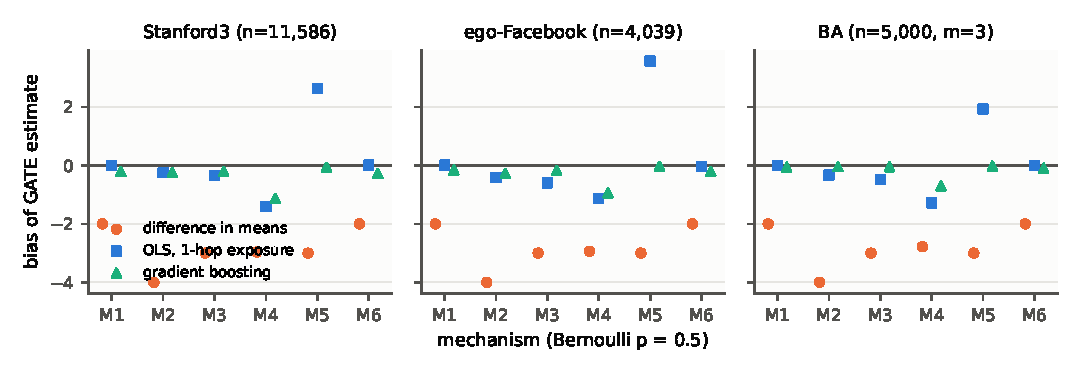
\includegraphics[width=\linewidth]{figures/fig_bias_by_mechanism.pdf}
\caption{Bias of the GATE estimate, Bernoulli($p=0.5$), 500 replications. Difference in means (orange) targets the direct effect and is biased by the spillover in every mechanism; the one-hop OLS (blue) is unbiased only under linear interference; gradient boosting (green) is accurate under the threshold response but not under linear response.}
\label{fig:bias}
\end{figure}

Table~\ref{tab:main} reports Stanford3 under Bernoulli($0.5$), and Figure~\ref{fig:bias} shows bias across all three graphs. Three patterns hold on every graph.

\textbf{The direct-effect estimators miss the GATE by the spillover.} The difference in means (DiM) has bias $-(\tau_m-1)$ in every mechanism, because the direct effect is 1 throughout. Under M1 it is $-2.00$, which is the spillover $2f_1$. The same holds for OLS on $(1,z,x)$. This is the most common practical error in network experiments.

\textbf{The one-hop regression is unbiased when the response is linear and biased otherwise.} Under M0, M1 and M6 the one-hop estimator has bias below $0.01$ in absolute value on Stanford3, and CR1 coverage of $0.94$--$0.96$. Under M2 (cubic) and M3 (saturating), the bias is $-0.25$ and $-0.34$, and coverage is at most $0.37$. Under M5 (threshold) the bias is $+2.63$. Quadratic exposure terms do not help at $p=0.5$ on these graphs: they reproduce the one-hop bias in Table~\ref{tab:main}. Gradient boosting is nearly unbiased under M5 ($-0.06$) but not under M1 ($-0.21$), and its bias under M1 grows to $-0.96$ at $p=0.1$ on Stanford3 (Table~\ref{tab:all}).

\textbf{Omitting the two-hop term is a large, predictable bias.} Under M4 the one-hop estimator has bias $-1.41$ on Stanford3, $-1.12$ on ego-Facebook, and $-1.28$ on BA, and its intervals never cover the GATE. The two-hop regression (R3) is unbiased on all three graphs (bias between $-0.01$ and $0.02$). Its standard error is much larger on the dense Stanford3 graph (SD $0.23$ against $0.06$). The reason is that the two-step exposure varies little there: its variance is $0.07$ times that of the one-hop exposure (\texttt{code/diag\_exposure.py}), so its coefficient is imprecisely estimated.

The two-hop bias has an exact form. Let $b$ and $c$ be the slopes from the linear projection of $f_2$ on $f_1$ and on $Z$ under Bernoulli assignment. Omitting $f_2$ from the one-hop regression gives a bias of $\gamma_2(b+c-1)$ for the GATE, where $\gamma_2=1.5$ is the two-hop coefficient. We estimated $b$ and $c$ by averaging 20 draws per graph (\texttt{code/diag\_omitted.py}). The predicted biases are $-1.41$ (Stanford3: $b=0.036$, $c=0.022$), $-1.13$ (ego-Facebook: $b=0.208$, $c=0.040$), and $-1.28$ (BA: $b=-0.001$, $c=0.148$). These match the simulated biases to within $0.01$. Clustering does not drive the bias. Stanford3 has clustering $0.24$ and BA has $0.009$, yet their biases are nearly equal, because the two-hop term loads on the direct-effect coefficient $c$ and on $b$, not on clustering as such.

\subsection{Design and inference}
\label{sec:design}

Table~\ref{tab:designs} (appendix) compares Bernoulli and graph-cluster (GCR) randomization on Stanford3. GCR changes the exposure distribution: units in the same community share treatment, so exposures are more dispersed. The share of units with one-hop exposure at most $0.1$ or at least $0.9$ rises from $6.5\%$ to $13.7\%$ on Stanford3, from $4.3\%$ to $63.7\%$ on ego-Facebook, and from $13.9\%$ to $24.4\%$ on BA (\texttt{code/diag\_exposure.py}). The effect on the threshold mechanism is large. At $p=0.5$, GCR cuts the one-hop bias from $2.63$ to $1.23$. At $p=0.1$, however, the one-hop bias is $-0.07$ under GCR but $1.03$ under the quadratic estimator, so the two misspecified models disagree and the apparent accuracy is cancellation. Agreement between two misspecified estimators is not evidence that either is correct. GCR also raises variance when outcomes share community shocks: under M6 at $p=0.5$, the SD is $0.39$ under GCR against $0.16$ under Bernoulli, because the number of independent units falls from $11{,}586$ to the number of communities ($427$).

\begin{figure}[t]
\centering
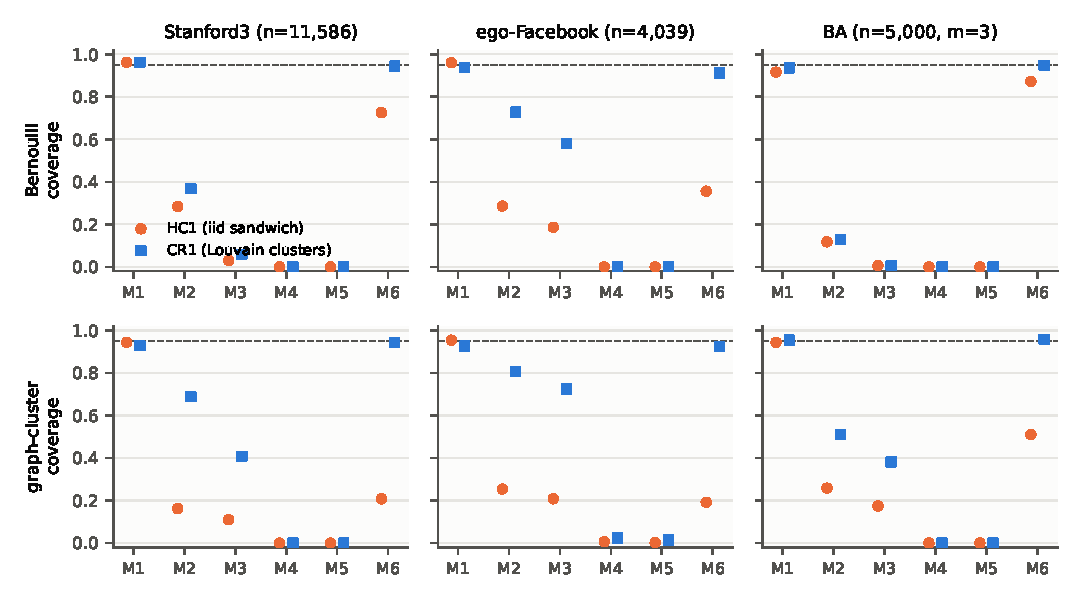
\includegraphics[width=\linewidth]{figures/fig_coverage.pdf}
\caption{Coverage of nominal 95\% intervals for the one-hop OLS, by mechanism, graph and design (Bernoulli top, graph-cluster bottom; $p=0.5$). HC1 is the iid sandwich; CR1 clusters on Louvain communities. Coverage near zero under misspecified mechanisms reflects bias, not variance.}
\label{fig:cov}
\end{figure}

Figure~\ref{fig:cov} shows coverage of nominal 95\% intervals. Under community shocks (M6) and Bernoulli assignment, HC1 covers $0.73$ on Stanford3, $0.87$ on BA and $0.36$ on ego-Facebook, while CR1 covers $0.94$, $0.95$ and $0.91$. Under GCR with $p=0.5$, HC1 falls to $0.21$, $0.51$ and $0.19$, and CR1 stays at $0.94$, $0.96$ and $0.92$. Without shocks, HC1 and CR1 are both close to nominal under M1. CR1 is not reliable when few clusters are treated: at GCR $p=0.1$ on ego-Facebook it covers $0.83$ under M1 and $0.76$ under M6.

\subsection{Degree, sample size and treatment probability}
\label{sec:scaling}

\begin{figure}[t]
\centering
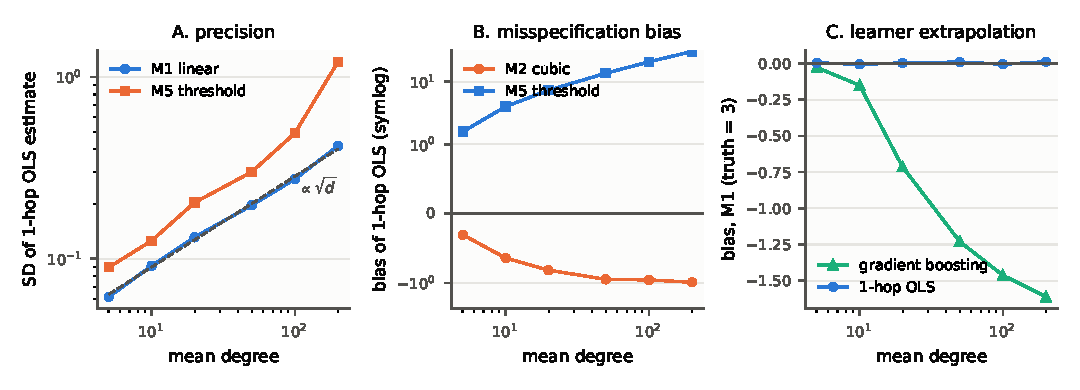
\includegraphics[width=\linewidth]{figures/fig_degree.pdf}
\caption{Degree sweep (E2; ER graphs, $n\approx5{,}000$, Bernoulli($0.5$)). A: SD of the one-hop estimate under M1 and M5 with a $\sqrt d$ reference. B: one-hop bias under M2 and M5. C: bias of gradient boosting and of the one-hop OLS under M1.}
\label{fig:degree}
\end{figure}

\textbf{Precision scales with the square root of degree.} Under M1 the SD of the one-hop estimate is $0.0275$--$0.0295$ times $\sqrt{d}$ at every degree from 5 to 200 (Figure~\ref{fig:degree}A). The slope on $f_1$ has variance proportional to $1/\mathrm{Var}(f_1)=d/\{p(1-p)\}$, so the SD is $\sqrt{d/(n\,p(1-p))}$, which gives $0.028\sqrt d$ at $n=5{,}000$ and $p=0.5$.

\textbf{The cubic bias saturates; the threshold bias grows with $\sqrt d$.} Under M2 the one-hop bias moves from $-0.31$ at degree 5 to $-0.99$ at degree 200. The limit $-1$ is the gap between the secant slope of $4f^3$ on $[0,1]$ (equal to 4) and its derivative at $p=1/2$ (equal to 3). Under M5 the bias grows from $+1.59$ at degree 5 to $+30.7$ at degree 200. For Bernoulli($1/2$) with $\sigma=0.5/\sqrt d$, the slope of $\mathbf 1\{f_1\ge 1/2\}$ on $f_1$ is $0.80\sqrt d$, so the predicted bias is $3\cdot0.80\sqrt d-3$. That gives $13.9$ at degree 50 (simulated $13.7$) and $30.8$ at degree 200 (simulated $30.7$). The linear fit extrapolates a step that is effectively located in a narrow band around the mean exposure, and the extrapolation distance grows as $\sqrt d$.

\textbf{Gradient boosting degrades with degree.} Under M1 its bias is $-0.03$ at degree 5 and $-1.61$ at degree 200 (Figure~\ref{fig:degree}C). Trees predict a constant beyond the range of the training data, so the all-treated point is predicted from the highest observed exposure bin.

\textbf{Misspecification bias does not vanish with the sample size.} Under M2, M3 and M5 the one-hop bias is essentially constant from $n=1{,}000$ to $n=16{,}000$ (Figure~\ref{fig:size}A): $-0.86$, $-0.84$ and $-0.84$ for M2; $-1.17$, $-1.15$, $-1.16$ for M3; $7.36$, $7.32$, $7.32$ for M5. The SD falls like $n^{-1/2}$ (Figure~\ref{fig:size}B), so coverage goes to zero. Gradient boosting on M1 is also inconsistent: its bias is $-1.03$, $-0.75$ and $-0.83$ at the three sample sizes.

\begin{figure}[t]
\centering
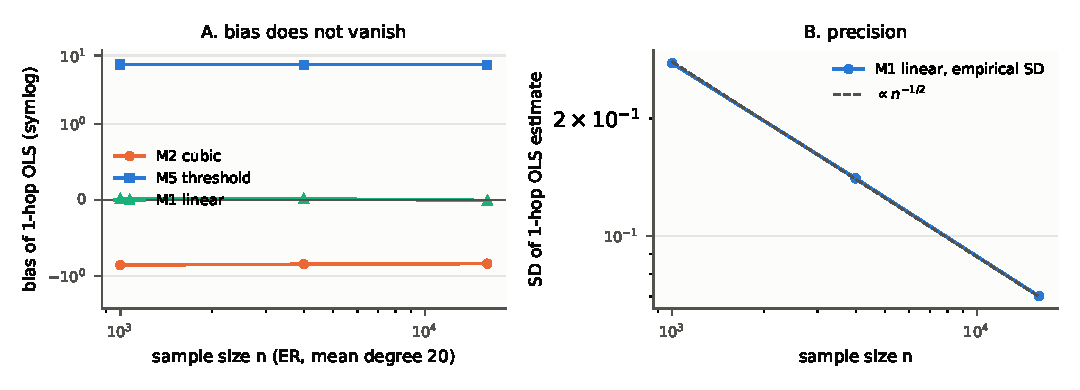
\includegraphics[width=\linewidth]{figures/fig_sample_size.pdf}
\caption{Sample-size sweep (E3; ER graphs, mean degree 20, Bernoulli($0.5$)). A: bias of the one-hop OLS under M1, M2 and M5 is stable in $n$ (M3 is in \texttt{summary\_E3.csv}). B: SD of the one-hop OLS under M1 falls like $n^{-1/2}$.}
\label{fig:size}
\end{figure}

\textbf{The sign of the bias depends on the treatment probability.} Figure~\ref{fig:p} plots bias against $p$ on ego-Facebook. The cubic bias is $-2.85$ at $p=0.1$, changes sign between $p=0.5$ ($-0.45$) and $p=0.7$ ($+1.42$), and is $+3.79$ at $p=0.9$. A first-order approximation predicts a zero crossing where the local slope $12p^2$ equals the secant slope 4, that is at $p=1/\sqrt3\approx 0.58$, consistent with the observed crossing. The saturating bias changes sign near $p=0.4$. The threshold bias is largest near $p=0.5$, where the cutoff lies in the bulk of the exposure distribution: it is $+3.58$ at $p=0.5$ and $-2.27$ at $p=0.9$. Gradient boosting is U-shaped in $p$ under M1 ($-1.10$ at $p=0.1$, $-0.15$ at $p=0.5$, $-1.13$ at $p=0.9$), consistent with extrapolation failure at both ends. Coverage under misspecification is not evidence of accuracy: M2 at $p=0.5$ on ego-Facebook has coverage $0.74$ with bias $-0.45$, because its SD across replications is $0.56$.

\begin{figure}[t]
\centering
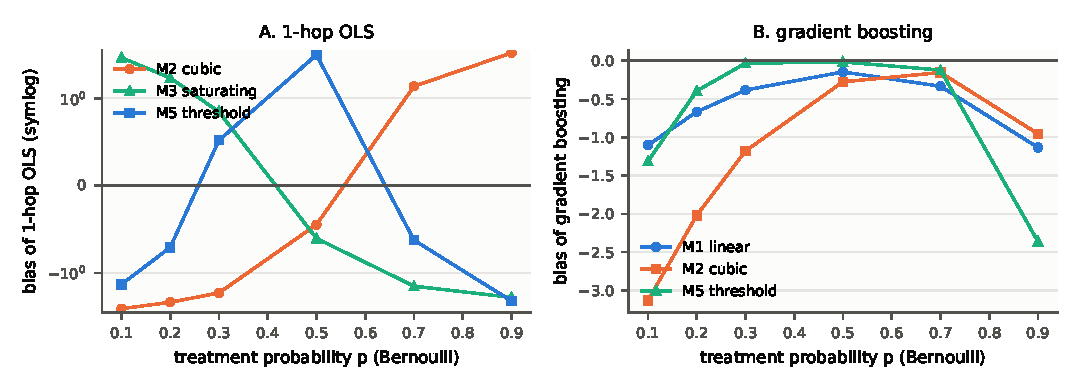
\includegraphics[width=\linewidth]{figures/fig_p_sweep.pdf}
\caption{Treatment-probability sweep (E4; ego-Facebook, Bernoulli). A: bias of the one-hop OLS for M2, M3 and M5 changes sign with $p$. B: bias of gradient boosting under M1, M2 and M5; the linear case is U-shaped.}
\label{fig:p}
\end{figure}

\section{Discussion and limitations}
\label{sec:discussion}
\paragraph{What this means for practice.} Three conclusions follow from these simulations. First, a platform that reports the difference in means or the direct-effect regression under interference is reporting the direct effect, and the gap to the GATE equals the spillover. Second, the one-hop regression of \citet{chin2019} is a valid GATE estimator only when the exposure response is linear over the range that the GATE extrapolates to. Nonlinearity cannot be diagnosed from the variance estimates, because misspecified intervals have near-zero coverage and are usually tight. Third, a sensitivity analysis is needed in addition to the standard error: the one-hop, two-hop, quadratic and flexible estimators can disagree by several units, and when they do, the disagreement is the diagnostic. A practical check is the distribution of observed exposures. If little mass lies near 0 or 1, the GATE is an extrapolation and should be reported with that caveat.

\paragraph{Design.} Graph-cluster randomization moves exposures toward the extremes and so reduces extrapolation bias for threshold-type responses, but it reduces the effective sample size to the number of communities. In our graphs that cost is large under community shocks and small under linear responses. The benefit at $p=0.1$ can be illusory (the cancellation described in Section~\ref{sec:design}), so design choices should be evaluated with the same sensitivity analysis.

\paragraph{Limitations.} Our conclusions are conditional on the setup. (1) Interference is exposure-based: outcomes depend on the treatment of neighbours and on their two-step exposure, but not on neighbours' outcomes, so equilibrium, contagion or feedback mechanisms are not studied. (2) The estimand is the finite-population GATE with known mean functions, which makes bias measurable but is an idealization of what an experimenter faces. (3) Outcomes are binary-treatment, Gaussian, with one covariate. (4) The graphs are at most 11{,}586 nodes; the largest-component reduction removes nodes that are not part of the giant component. (5) We use one walk-based two-step exposure, not the exact two-hop share, and the two-hop identity in Section~\ref{sec:main} is derived for that exposure. (6) Inference uses sandwich variances and Louvain clusters. We did not evaluate the block or cluster bootstrap of \citet{chin2019} and \citet{han2023}, which may behave differently. (7) Gradient boosting uses fixed hyperparameters and no tuning, so the flexible-learner results reflect one configuration. (8) The number of replications (500) gives Monte Carlo standard errors for bias with median $0.006$ and maximum $0.13$ across settings (listed in the summary files), which separates the effects reported here but not finer ones. (9) E4 at $p\in\{0.1,0.3,0.5\}$ repeats E1 with independent seeds; the two agree within Monte Carlo error ($|z|\le 2.2$ for all 36 shared estimator-settings).

\paragraph{Negative and unexpected results.} We did not find that clustering drives the two-hop bias, which contradicted our initial expectation. Quadratic exposure terms did not correct the cubic bias at $p=0.5$. Gradient boosting was more accurate than the one-hop regression under the threshold mechanism, but less accurate under linear and smooth mechanisms at extreme $p$ and at high degree. The threshold bias grows with $\sqrt d$, so denser networks make the naive regression worse, not better.

\begin{ack}
Funding and competing interests: none declared. The simulations were run on a shared 4-CPU compute quota; no external data or services were used beyond the public graphs cited in Section~\ref{sec:setup}.
\end{ack}

\bibliographystyle{plainnat}
\bibliography{refs}

\newpage
\appendix
\section{Reproducibility details}
\label{app:repro}
Every number in the paper is generated by the scripts in the repository; \texttt{README.md} gives the environment, data sources and checksums, the commands, and the runtime. The main steps are: \texttt{prepare\_graphs.py} (graphs and Louvain partitions, \texttt{graph\_stats.csv}); \texttt{run\_all.sh} (E1--E4, 500 replications per setting, master seed 20261114); \texttt{analyze.py} (summaries); \texttt{make\_tables.py} and \texttt{make\_figures.py} (LaTeX tables and figures); \texttt{diag\_omitted.py} (projection slopes for the two-hop identity); and \texttt{diag\_exposure.py} (exposure dispersion, Section~\ref{sec:design}). The per-replication outputs are in \texttt{results/raw/}.

{\footnotesize\begin{longtable}{lllrrrrrrr}
\caption{Every E1 setting: bias and coverage for the one-hop OLS, the quadratic OLS (quad.), and gradient boosting (GBM). Design: B = Bernoulli, C = graph-cluster randomization, followed by $p$. Coverage is for nominal 95\% intervals (HC1 and CR1); GBM has no interval. Truth is the GATE in Table~\ref{tab:mech}.} \label{tab:all}\\
\toprule
Graph & Mech. & Design, $p$ & DiM bias & OLS bias & OLS SD & cov.\ HC1 & cov.\ CR1 & quad.\ bias & GBM bias \\
\midrule
\endfirsthead
\multicolumn{10}{l}{\small Table \ref{tab:all} continued} \\
\toprule
Graph & Mech. & Design, $p$ & DiM bias & OLS bias & OLS SD & cov.\ HC1 & cov.\ CR1 & quad.\ bias & GBM bias \\
\midrule
\endhead
\bottomrule
\endfoot
Stanford3 & M0 & B, 0.1 & -0.00 & -0.01 & 0.11 & 0.94 & 0.93 & -0.01 & -0.05 \\
Stanford3 & M0 & B, 0.3 & 0.00 & -0.01 & 0.07 & 0.96 & 0.95 & -0.00 & -0.03 \\
Stanford3 & M0 & B, 0.5 & 0.00 & 0.00 & 0.06 & 0.96 & 0.96 & 0.00 & -0.02 \\
Stanford3 & M0 & C, 0.1 & 0.00 & -0.00 & 0.08 & 0.94 & 0.90 & -0.01 & -0.03 \\
Stanford3 & M0 & C, 0.5 & 0.00 & 0.00 & 0.04 & 0.96 & 0.95 & 0.00 & -0.02 \\
Stanford3 & M1 & B, 0.1 & -2.00 & -0.01 & 0.11 & 0.96 & 0.95 & -0.01 & -0.96 \\
Stanford3 & M1 & B, 0.3 & -2.01 & -0.00 & 0.07 & 0.96 & 0.96 & -0.00 & -0.35 \\
Stanford3 & M1 & B, 0.5 & -2.00 & 0.00 & 0.06 & 0.96 & 0.96 & 0.00 & -0.21 \\
Stanford3 & M1 & C, 0.1 & -1.29 & 0.00 & 0.07 & 0.95 & 0.93 & 0.01 & -0.22 \\
Stanford3 & M1 & C, 0.5 & -1.28 & -0.00 & 0.04 & 0.94 & 0.93 & -0.00 & -0.08 \\
Stanford3 & M2 & B, 0.1 & -4.00 & -1.75 & 0.17 & 0.00 & 0.00 & -0.16 & -1.70 \\
Stanford3 & M2 & B, 0.3 & -4.00 & -1.13 & 0.12 & 0.00 & 0.00 & -0.23 & -0.53 \\
Stanford3 & M2 & B, 0.5 & -4.00 & -0.25 & 0.12 & 0.28 & 0.37 & -0.25 & -0.23 \\
Stanford3 & M2 & C, 0.1 & -3.34 & -1.68 & 0.31 & 0.00 & 0.00 & -0.29 & -0.56 \\
Stanford3 & M2 & C, 0.5 & -2.72 & -0.27 & 0.36 & 0.16 & 0.69 & -0.30 & -0.08 \\
Stanford3 & M3 & B, 0.1 & -3.00 & 1.92 & 0.20 & 0.00 & 0.00 & -0.36 & -0.69 \\
Stanford3 & M3 & B, 0.3 & -3.00 & 0.52 & 0.12 & 0.00 & 0.01 & -0.39 & -0.23 \\
Stanford3 & M3 & B, 0.5 & -3.00 & -0.34 & 0.09 & 0.03 & 0.06 & -0.34 & -0.20 \\
Stanford3 & M3 & C, 0.1 & -1.39 & 1.43 & 0.46 & 0.00 & 0.09 & -0.50 & -0.12 \\
Stanford3 & M3 & C, 0.5 & -2.17 & -0.42 & 0.26 & 0.11 & 0.41 & -0.42 & -0.07 \\
Stanford3 & M4 & B, 0.1 & -2.97 & -1.41 & 0.10 & 0.00 & 0.00 & -1.46 & -2.01 \\
Stanford3 & M4 & B, 0.3 & -2.97 & -1.40 & 0.07 & 0.00 & 0.00 & -1.41 & -1.28 \\
Stanford3 & M4 & B, 0.5 & -2.97 & -1.41 & 0.06 & 0.00 & 0.00 & -1.41 & -1.13 \\
Stanford3 & M4 & C, 0.1 & -2.22 & -0.80 & 0.15 & 0.00 & 0.00 & -0.80 & -0.79 \\
Stanford3 & M4 & C, 0.5 & -2.20 & -0.76 & 0.05 & 0.00 & 0.00 & -0.77 & -0.35 \\
Stanford3 & M5 & B, 0.1 & -3.00 & -0.56 & 0.14 & 0.02 & 0.04 & 0.57 & -1.21 \\
Stanford3 & M5 & B, 0.3 & -3.00 & 0.30 & 0.11 & 0.16 & 0.25 & 1.00 & -0.12 \\
Stanford3 & M5 & B, 0.5 & -3.00 & 2.63 & 0.09 & 0.00 & 0.00 & 2.63 & -0.06 \\
Stanford3 & M5 & C, 0.1 & -2.07 & -0.07 & 0.37 & 0.39 & 0.85 & 1.03 & -0.07 \\
Stanford3 & M5 & C, 0.5 & -0.79 & 1.23 & 0.10 & 0.00 & 0.00 & 1.27 & -0.04 \\
Stanford3 & M6 & B, 0.1 & -2.00 & 0.01 & 0.27 & 0.71 & 0.95 & 0.01 & -1.01 \\
Stanford3 & M6 & B, 0.3 & -2.00 & -0.00 & 0.16 & 0.79 & 0.94 & 0.00 & -0.42 \\
Stanford3 & M6 & B, 0.5 & -2.00 & 0.01 & 0.16 & 0.73 & 0.94 & 0.01 & -0.27 \\
Stanford3 & M6 & C, 0.1 & -1.30 & -0.01 & 0.51 & 0.29 & 0.88 & -0.01 & -0.25 \\
Stanford3 & M6 & C, 0.5 & -1.27 & 0.03 & 0.39 & 0.21 & 0.94 & 0.03 & -0.02 \\
ego-Facebook & M0 & B, 0.1 & -0.00 & -0.01 & 0.20 & 0.94 & 0.91 & -0.02 & -0.03 \\
ego-Facebook & M0 & B, 0.3 & 0.00 & 0.00 & 0.12 & 0.96 & 0.93 & 0.01 & -0.02 \\
ego-Facebook & M0 & B, 0.5 & 0.00 & 0.00 & 0.11 & 0.96 & 0.94 & 0.00 & -0.01 \\
ego-Facebook & M0 & C, 0.1 & 0.01 & 0.00 & 0.11 & 0.95 & 0.87 & 0.01 & -0.01 \\
ego-Facebook & M0 & C, 0.5 & -0.00 & -0.00 & 0.04 & 0.96 & 0.94 & -0.00 & 0.02 \\
ego-Facebook & M1 & B, 0.1 & -2.00 & -0.00 & 0.19 & 0.95 & 0.93 & 0.01 & -1.09 \\
ego-Facebook & M1 & B, 0.3 & -2.00 & -0.01 & 0.12 & 0.96 & 0.94 & -0.01 & -0.36 \\
ego-Facebook & M1 & B, 0.5 & -2.00 & 0.01 & 0.11 & 0.96 & 0.94 & 0.01 & -0.16 \\
ego-Facebook & M1 & C, 0.1 & -0.59 & -0.00 & 0.09 & 0.94 & 0.83 & -0.01 & -0.07 \\
ego-Facebook & M1 & C, 0.5 & -0.53 & 0.00 & 0.04 & 0.95 & 0.93 & 0.00 & 0.01 \\
ego-Facebook & M2 & B, 0.1 & -3.99 & -2.88 & 0.67 & 0.00 & 0.00 & -0.84 & -3.18 \\
ego-Facebook & M2 & B, 0.3 & -4.00 & -1.80 & 0.53 & 0.00 & 0.02 & -0.46 & -1.20 \\
ego-Facebook & M2 & B, 0.5 & -4.00 & -0.41 & 0.55 & 0.29 & 0.73 & -0.46 & -0.28 \\
ego-Facebook & M2 & C, 0.1 & -1.84 & -0.91 & 0.53 & 0.00 & 0.27 & -0.23 & -0.31 \\
ego-Facebook & M2 & C, 0.5 & -1.18 & -0.11 & 0.28 & 0.25 & 0.81 & -0.11 & -0.00 \\
ego-Facebook & M3 & B, 0.1 & -3.00 & 3.34 & 1.03 & 0.00 & 0.01 & -1.77 & -0.67 \\
ego-Facebook & M3 & B, 0.3 & -3.00 & 0.84 & 0.57 & 0.14 & 0.55 & -0.80 & -0.13 \\
ego-Facebook & M3 & B, 0.5 & -3.00 & -0.60 & 0.42 & 0.19 & 0.58 & -0.63 & -0.17 \\
ego-Facebook & M3 & C, 0.1 & -0.55 & 0.72 & 0.67 & 0.05 & 0.49 & -0.33 & -0.02 \\
ego-Facebook & M3 & C, 0.5 & -0.98 & -0.18 & 0.22 & 0.21 & 0.72 & -0.18 & 0.01 \\
ego-Facebook & M4 & B, 0.1 & -2.94 & -1.12 & 0.20 & 0.00 & 0.00 & -1.41 & -1.92 \\
ego-Facebook & M4 & B, 0.3 & -2.94 & -1.12 & 0.12 & 0.00 & 0.00 & -1.16 & -1.16 \\
ego-Facebook & M4 & B, 0.5 & -2.94 & -1.12 & 0.11 & 0.00 & 0.00 & -1.11 & -0.94 \\
ego-Facebook & M4 & C, 0.1 & -1.03 & -0.20 & 0.12 & 0.32 & 0.32 & -0.21 & -0.17 \\
ego-Facebook & M4 & C, 0.5 & -0.97 & -0.19 & 0.05 & 0.01 & 0.02 & -0.19 & -0.01 \\
ego-Facebook & M5 & B, 0.1 & -3.01 & -1.42 & 0.68 & 0.06 & 0.38 & 2.34 & -1.39 \\
ego-Facebook & M5 & B, 0.3 & -3.00 & 0.49 & 0.60 & 0.31 & 0.63 & 2.30 & -0.03 \\
ego-Facebook & M5 & B, 0.5 & -3.00 & 3.57 & 0.24 & 0.00 & 0.00 & 3.90 & -0.03 \\
ego-Facebook & M5 & C, 0.1 & -0.64 & 0.12 & 0.37 & 0.40 & 0.64 & 0.40 & -0.04 \\
ego-Facebook & M5 & C, 0.5 & -0.33 & 0.30 & 0.07 & 0.00 & 0.01 & 0.31 & -0.00 \\
ego-Facebook & M6 & B, 0.1 & -2.00 & 0.03 & 0.90 & 0.42 & 0.89 & -0.06 & -1.14 \\
ego-Facebook & M6 & B, 0.3 & -2.00 & -0.01 & 0.59 & 0.40 & 0.90 & -0.03 & -0.41 \\
ego-Facebook & M6 & B, 0.5 & -2.00 & -0.03 & 0.59 & 0.36 & 0.91 & -0.03 & -0.21 \\
ego-Facebook & M6 & C, 0.1 & -0.58 & 0.02 & 0.76 & 0.21 & 0.76 & 0.02 & -0.08 \\
ego-Facebook & M6 & C, 0.5 & -0.54 & 0.00 & 0.43 & 0.19 & 0.92 & 0.01 & 0.04 \\
BA & M0 & B, 0.1 & -0.00 & 0.00 & 0.11 & 0.95 & 0.94 & 0.00 & -0.02 \\
BA & M0 & B, 0.3 & -0.00 & 0.00 & 0.07 & 0.94 & 0.94 & 0.00 & -0.02 \\
BA & M0 & B, 0.5 & -0.00 & 0.00 & 0.07 & 0.95 & 0.94 & 0.00 & 0.00 \\
BA & M0 & C, 0.1 & 0.00 & 0.01 & 0.08 & 0.95 & 0.94 & 0.02 & 0.02 \\
BA & M0 & C, 0.5 & 0.00 & 0.00 & 0.05 & 0.95 & 0.95 & 0.00 & 0.00 \\
BA & M1 & B, 0.1 & -2.00 & 0.00 & 0.11 & 0.94 & 0.94 & -0.00 & -0.91 \\
BA & M1 & B, 0.3 & -2.00 & -0.00 & 0.07 & 0.94 & 0.95 & -0.00 & -0.14 \\
BA & M1 & B, 0.5 & -2.00 & -0.00 & 0.07 & 0.92 & 0.94 & -0.00 & -0.06 \\
BA & M1 & C, 0.1 & -1.11 & 0.00 & 0.08 & 0.96 & 0.95 & -0.00 & -0.12 \\
BA & M1 & C, 0.5 & -1.11 & 0.00 & 0.05 & 0.94 & 0.95 & 0.00 & 0.00 \\
BA & M2 & B, 0.1 & -4.00 & -3.17 & 0.12 & 0.00 & 0.00 & -0.95 & -3.11 \\
BA & M2 & B, 0.3 & -4.00 & -1.90 & 0.12 & 0.00 & 0.00 & -0.47 & -0.31 \\
BA & M2 & B, 0.5 & -4.00 & -0.33 & 0.14 & 0.12 & 0.13 & -0.33 & -0.05 \\
BA & M2 & C, 0.1 & -3.27 & -2.45 & 0.17 & 0.00 & 0.00 & -0.46 & -0.54 \\
BA & M2 & C, 0.5 & -2.38 & -0.22 & 0.32 & 0.26 & 0.51 & -0.22 & -0.00 \\
BA & M3 & B, 0.1 & -3.00 & 3.19 & 0.17 & 0.00 & 0.00 & -1.58 & -0.42 \\
BA & M3 & B, 0.3 & -3.01 & 1.10 & 0.14 & 0.00 & 0.00 & -0.70 & -0.05 \\
BA & M3 & B, 0.5 & -3.00 & -0.48 & 0.12 & 0.01 & 0.01 & -0.47 & -0.05 \\
BA & M3 & C, 0.1 & -0.92 & 2.15 & 0.23 & 0.00 & 0.00 & -0.66 & -0.03 \\
BA & M3 & C, 0.5 & -1.88 & -0.29 & 0.22 & 0.17 & 0.38 & -0.31 & -0.01 \\
BA & M4 & B, 0.1 & -2.78 & -1.28 & 0.11 & 0.00 & 0.00 & -1.28 & -1.70 \\
BA & M4 & B, 0.3 & -2.78 & -1.28 & 0.07 & 0.00 & 0.00 & -1.28 & -0.89 \\
BA & M4 & B, 0.5 & -2.78 & -1.28 & 0.06 & 0.00 & 0.00 & -1.28 & -0.70 \\
BA & M4 & C, 0.1 & -1.93 & -0.89 & 0.09 & 0.00 & 0.00 & -0.91 & -0.80 \\
BA & M4 & C, 0.5 & -1.93 & -0.89 & 0.05 & 0.00 & 0.00 & -0.89 & -0.39 \\
BA & M5 & B, 0.1 & -3.00 & -1.35 & 0.20 & 0.00 & 0.00 & 4.57 & -0.48 \\
BA & M5 & B, 0.3 & -3.00 & 1.22 & 0.14 & 0.00 & 0.00 & 2.83 & 0.01 \\
BA & M5 & B, 0.5 & -3.00 & 1.93 & 0.09 & 0.00 & 0.00 & 1.94 & -0.02 \\
BA & M5 & C, 0.1 & -1.43 & -0.20 & 0.20 & 0.49 & 0.92 & 2.21 & 0.01 \\
BA & M5 & C, 0.5 & -0.84 & 1.05 & 0.08 & 0.00 & 0.00 & 1.09 & -0.00 \\
BA & M6 & B, 0.1 & -2.00 & 0.01 & 0.20 & 0.84 & 0.94 & -0.02 & -0.88 \\
BA & M6 & B, 0.3 & -2.00 & 0.00 & 0.13 & 0.88 & 0.94 & -0.00 & -0.19 \\
BA & M6 & B, 0.5 & -2.00 & -0.01 & 0.12 & 0.87 & 0.95 & -0.01 & -0.09 \\
BA & M6 & C, 0.1 & -1.11 & 0.00 & 0.33 & 0.52 & 0.93 & -0.00 & -0.11 \\
BA & M6 & C, 0.5 & -1.11 & -0.00 & 0.19 & 0.51 & 0.96 & -0.00 & -0.02 \\
\end{longtable}
}

\begin{table}[h]
\caption{Bernoulli versus graph-cluster randomization on Stanford3 for the one-hop OLS and the quadratic OLS. Cluster coverage is CR1 and the target is the GATE.}
\label{tab:designs}
\centering
\small
\begin{tabular}{llrrrrrr}
\toprule
 & & \multicolumn{4}{c}{OLS, 1-hop ($z,f_1$)} & \multicolumn{2}{c}{OLS, quad.} \\
\cmidrule(lr){3-6}\cmidrule(lr){7-8}
Mechanism & Design & bias & SD & RMSE & cov.\ CR1 & bias & SD \\
\midrule
M1 linear & Bernoulli, $p=0.1$ & -0.01 & 0.11 & 0.11 & 0.95 & -0.01 & 0.14 \\
M1 linear & graph-cluster, $p=0.1$ & 0.00 & 0.07 & 0.07 & 0.93 & 0.01 & 0.10 \\
M1 linear & Bernoulli, $p=0.5$ & 0.00 & 0.06 & 0.06 & 0.96 & 0.00 & 0.06 \\
M1 linear & graph-cluster, $p=0.5$ & -0.00 & 0.04 & 0.04 & 0.93 & -0.00 & 0.04 \\
\midrule
M2 cubic & Bernoulli, $p=0.1$ & -1.75 & 0.17 & 1.75 & 0.00 & -0.16 & 0.14 \\
M2 cubic & graph-cluster, $p=0.1$ & -1.68 & 0.31 & 1.71 & 0.00 & -0.29 & 0.11 \\
M2 cubic & Bernoulli, $p=0.5$ & -0.25 & 0.12 & 0.28 & 0.37 & -0.25 & 0.06 \\
M2 cubic & graph-cluster, $p=0.5$ & -0.27 & 0.36 & 0.45 & 0.69 & -0.30 & 0.04 \\
\midrule
M3 saturating & Bernoulli, $p=0.1$ & 1.92 & 0.20 & 1.93 & 0.00 & -0.36 & 0.15 \\
M3 saturating & graph-cluster, $p=0.1$ & 1.43 & 0.46 & 1.50 & 0.09 & -0.50 & 0.13 \\
M3 saturating & Bernoulli, $p=0.5$ & -0.34 & 0.09 & 0.35 & 0.06 & -0.34 & 0.06 \\
M3 saturating & graph-cluster, $p=0.5$ & -0.42 & 0.26 & 0.50 & 0.41 & -0.42 & 0.04 \\
\midrule
M5 threshold & Bernoulli, $p=0.1$ & -0.56 & 0.14 & 0.58 & 0.04 & 0.57 & 0.16 \\
M5 threshold & graph-cluster, $p=0.1$ & -0.07 & 0.37 & 0.38 & 0.85 & 1.03 & 0.29 \\
M5 threshold & Bernoulli, $p=0.5$ & 2.63 & 0.09 & 2.63 & 0.00 & 2.63 & 0.09 \\
M5 threshold & graph-cluster, $p=0.5$ & 1.23 & 0.10 & 1.23 & 0.00 & 1.27 & 0.09 \\
\midrule
M6 shocks & Bernoulli, $p=0.1$ & 0.01 & 0.27 & 0.27 & 0.95 & 0.01 & 0.24 \\
M6 shocks & graph-cluster, $p=0.1$ & -0.01 & 0.51 & 0.51 & 0.88 & -0.01 & 0.53 \\
M6 shocks & Bernoulli, $p=0.5$ & 0.01 & 0.16 & 0.16 & 0.94 & 0.01 & 0.15 \\
M6 shocks & graph-cluster, $p=0.5$ & 0.03 & 0.39 & 0.39 & 0.94 & 0.03 & 0.38 \\
\bottomrule
\end{tabular}

\end{table}

\section*{NeurIPS Paper Checklist}

%%% BEGIN INSTRUCTIONS %%%
The checklist is designed to encourage best practices for responsible machine learning research, addressing issues of reproducibility, transparency, research ethics, and societal impact. Do not remove the checklist: {\bf The papers not including the checklist will be desk rejected.} The checklist should follow the references and follow the (optional) supplemental material.  The checklist does NOT count towards the page
limit. 

Please read the checklist guidelines carefully for information on how to answer these questions. For each question in the checklist:
\begin{itemize}
    \item You should answer \answerYes{}, \answerNo{}, or \answerNA{}.
    \item \answerNA{} means either that the question is Not Applicable for that particular paper or the relevant information is Not Available.
    \item Please provide a short (1--2 sentence) justification right after your answer (even for \answerNA). 
   % \item {\bf The papers not including the checklist will be desk rejected.}
\end{itemize}

{\bf The checklist answers are an integral part of your paper submission.} They are visible to the reviewers, area chairs, senior area chairs, and ethics reviewers. You will also be asked to include it (after eventual revisions) with the final version of your paper, and its final version will be published with the paper.

The reviewers of your paper will be asked to use the checklist as one of the factors in their evaluation. While \answerYes{} is generally preferable to \answerNo{}, it is perfectly acceptable to answer \answerNo{} provided a proper justification is given (e.g., error bars are not reported because it would be too computationally expensive'' or ``we were unable to find the license for the dataset we used''). In general, answering \answerNo{} or \answerNA{} is not grounds for rejection. While the questions are phrased in a binary way, we acknowledge that the true answer is often more nuanced, so please just use your best judgment and write a justification to elaborate. All supporting evidence can appear either in the main paper or the supplemental material, provided in appendix. If you answer \answerYes{} to a question, in the justification please point to the section(s) where related material for the question can be found.

IMPORTANT, please:
\begin{itemize}
    \item {\bf Delete this instruction block, but keep the section heading ``NeurIPS Paper Checklist"},
    \item  {\bf Keep the checklist subsection headings, questions/answers and guidelines below.}
    \item {\bf Do not modify the questions and only use the provided macros for your answers}.
\end{itemize} 
 

%%% END INSTRUCTIONS %%%


\begin{enumerate}

\item {\bf Claims}
    \item[] Question: Do the main claims made in the abstract and introduction accurately reflect the paper's contributions and scope?
    \item[] Answer: \answerYes{}
    \item[] Justification: The abstract and introduction state the claims that Sections~\ref{sec:main}--\ref{sec:scaling} test (direct-effect bias, one-hop bias under nonlinear interference, two-hop omission, inference under shocks, degree/sample-size/treatment-probability dependence), and the scope is limited to exposure-based interference as stated in Section~\ref{sec:discussion}.
    \item[] Guidelines:
    \begin{itemize}
        \item The answer \answerNA{} means that the abstract and introduction do not include the claims made in the paper.
        \item The abstract and/or introduction should clearly state the claims made, including the contributions made in the paper and important assumptions and limitations. A \answerNo{} or \answerNA{} answer to this question will not be perceived well by the reviewers. 
        \item The claims made should match theoretical and experimental results, and reflect how much the results can be expected to generalize to other settings. 
        \item It is fine to include aspirational goals as motivation as long as it is clear that these goals are not attained by the paper. 
    \end{itemize}

\item {\bf Limitations}
    \item[] Question: Does the paper discuss the limitations of the work performed by the authors?
    \item[] Answer: \answerYes{}
    \item[] Justification: Section~\ref{sec:discussion} lists nine limitations, including the restriction to exposure-based interference, the finite-population GATE with known mean functions, Gaussian outcomes, the walk-based two-step exposure, the untested bootstrap alternatives, the fixed untuned learner, and the Monte Carlo precision.
    \item[] Guidelines:
    \begin{itemize}
        \item The answer \answerNA{} means that the paper has no limitation while the answer \answerNo{} means that the paper has limitations, but those are not discussed in the paper. 
        \item The authors are encouraged to create a separate ``Limitations'' section in their paper.
        \item The paper should point out any strong assumptions and how robust the results are to violations of these assumptions (e.g., independence assumptions, noiseless settings, model well-specification, asymptotic approximations only holding locally). The authors should reflect on how these assumptions might be violated in practice and what the implications would be.
        \item The authors should reflect on the scope of the claims made, e.g., if the approach was only tested on a few datasets or with a few runs. In general, empirical results often depend on implicit assumptions, which should be articulated.
        \item The authors should reflect on the factors that influence the performance of the approach. For example, a facial recognition algorithm may perform poorly when image resolution is low or images are taken in low lighting. Or a speech-to-text system might not be used reliably to provide closed captions for online lectures because it fails to handle technical jargon.
        \item The authors should discuss the computational efficiency of the proposed algorithms and how they scale with dataset size.
        \item If applicable, the authors should discuss possible limitations of their approach to address problems of privacy and fairness.
        \item While the authors might fear that complete honesty about limitations might be used by reviewers as grounds for rejection, a worse outcome might be that reviewers discover limitations that aren't acknowledged in the paper. The authors should use their best judgment and recognize that individual actions in favor of transparency play an important role in developing norms that preserve the integrity of the community. Reviewers will be specifically instructed to not penalize honesty concerning limitations.
    \end{itemize}

\item {\bf Theory assumptions and proofs}
    \item[] Question: For each theoretical result, does the paper provide the full set of assumptions and a complete (and correct) proof?
    \item[] Answer: \answerNA{}
    \item[] Justification: The paper contains no theorems. The two-hop identity and the large-degree approximations in Sections~\ref{sec:main} and \ref{sec:scaling} are first-order heuristic derivations, labelled as approximations and checked against the simulations; they are not presented as results with proofs.
    \item[] Guidelines:
    \begin{itemize}
        \item The answer \answerNA{} means that the paper does not include theoretical results. 
        \item All the theorems, formulas, and proofs in the paper should be numbered and cross-referenced.
        \item All assumptions should be clearly stated or referenced in the statement of any theorems.
        \item The proofs can either appear in the main paper or the supplemental material, but if they appear in the supplemental material, the authors are encouraged to provide a short proof sketch to provide intuition. 
        \item Inversely, any informal proof provided in the core of the paper should be complemented by formal proofs provided in appendix or supplemental material.
        \item Theorems and Lemmas that the proof relies upon should be properly referenced. 
    \end{itemize}

    \item {\bf Experimental result reproducibility}
    \item[] Question: Does the paper fully disclose all the information needed to reproduce the main experimental results of the paper to the extent that it affects the main claims and/or conclusions of the paper (regardless of whether the code and data are provided or not)?
    \item[] Answer: \answerYes{}
    \item[] Justification: The setup, estimators, designs, mechanisms, seeds and runtime are in Sections~\ref{sec:setup} and \ref{sec:experiments}, and Appendix~\ref{app:repro} points to the README with commands, environment and data checksums. Every simulated table and figure is generated by the scripts described there.
    \item[] Guidelines:
    \begin{itemize}
        \item The answer \answerNA{} means that the paper does not include experiments.
        \item If the paper includes experiments, a \answerNo{} answer to this question will not be perceived well by the reviewers: Making the paper reproducible is important, regardless of whether the code and data are provided or not.
        \item If the contribution is a dataset and\slash or model, the authors should describe the steps taken to make their results reproducible or verifiable. 
        \item Depending on the contribution, reproducibility can be accomplished in various ways. For example, if the contribution is a novel architecture, describing the architecture fully might suffice, or if the contribution is a specific model and empirical evaluation, it may be necessary to either make it possible for others to replicate the model with the same dataset, or provide access to the model. In general. releasing code and data is often one good way to accomplish this, but reproducibility can also be provided via detailed instructions for how to replicate the results, access to a hosted model (e.g., in the case of a large language model), releasing of a model checkpoint, or other means that are appropriate to the research performed.
        \item While NeurIPS does not require releasing code, the conference does require all submissions to provide some reasonable avenue for reproducibility, which may depend on the nature of the contribution. For example
        \begin{enumerate}
            \item If the contribution is primarily a new algorithm, the paper should make it clear how to reproduce that algorithm.
            \item If the contribution is primarily a new model architecture, the paper should describe the architecture clearly and fully.
            \item If the contribution is a new model (e.g., a large language model), then there should either be a way to access this model for reproducing the results or a way to reproduce the model (e.g., with an open-source dataset or instructions for how to construct the dataset).
            \item We recognize that reproducibility may be tricky in some cases, in which case authors are welcome to describe the particular way they provide for reproducibility. In the case of closed-source models, it may be that access to the model is limited in some way (e.g., to registered users), but it should be possible for other researchers to have some path to reproducing or verifying the results.
        \end{enumerate}
    \end{itemize}


\item {\bf Open access to data and code}
    \item[] Question: Does the paper provide open access to the data and code, with sufficient instructions to faithfully reproduce the main experimental results, as described in supplemental material?
    \item[] Answer: \answerYes{}
    \item[] Justification: The code, the README with the environment, data sources and checksums, and the generated summary CSVs are part of the submission package. Both graphs are public: Stanford3 from the Network Data Repository, and ego-Facebook from SNAP.
    \item[] Guidelines:
    \begin{itemize}
        \item The answer \answerNA{} means that paper does not include experiments requiring code.
        \item Please see the NeurIPS code and data submission guidelines (\url{https://neurips.cc/public/guides/CodeSubmissionPolicy}) for more details.
        \item While we encourage the release of code and data, we understand that this might not be possible, so \answerNo{} is an acceptable answer. Papers cannot be rejected simply for not including code, unless this is central to the contribution (e.g., for a new open-source benchmark).
        \item The instructions should contain the exact command and environment needed to run to reproduce the results. See the NeurIPS code and data submission guidelines (\url{https://neurips.cc/public/guides/CodeSubmissionPolicy}) for more details.
        \item The authors should provide instructions on data access and preparation, including how to access the raw data, preprocessed data, intermediate data, and generated data, etc.
        \item The authors should provide scripts to reproduce all experimental results for the new proposed method and baselines. If only a subset of experiments are reproducible, they should state which ones are omitted from the script and why.
        \item At submission time, to preserve anonymity, the authors should release anonymized versions (if applicable).
        \item Providing as much information as possible in supplemental material (appended to the paper) is recommended, but including URLs to data and code is permitted.
    \end{itemize}


\item {\bf Experimental setting/details}
    \item[] Question: Does the paper specify all the training and test details (e.g., data splits, hyperparameters, how they were chosen, type of optimizer) necessary to understand the results?
    \item[] Answer: \answerYes{}
    \item[] Justification: Graphs and their preprocessing are described in Section~\ref{sec:setup}. Designs, mechanisms, exposures, estimators and the gradient-boosting settings are specified there and in the code. Hyperparameters were fixed in advance and were not tuned.
    \item[] Guidelines:
    \begin{itemize}
        \item The answer \answerNA{} means that the paper does not include experiments.
        \item The experimental setting should be presented in the core of the paper to a level of detail that is necessary to appreciate the results and make sense of them.
        \item The full details can be provided either with the code, in appendix, or as supplemental material.
    \end{itemize}

\item {\bf Experiment statistical significance}
    \item[] Question: Does the paper report error bars suitably and correctly defined or other appropriate information about the statistical significance of the experiments?
    \item[] Answer: \answerYes{}
    \item[] Justification: Each setting uses 500 independent replications. Tables and figures report SDs, Monte Carlo standard errors for bias (in the summary CSVs; between 0.002 and 0.13 for bias with 500 replications), and coverage of nominal 95\% intervals. Figures show point estimates without error bars, so the Monte Carlo errors are in the summary CSVs rather than the figures.
    \item[] Guidelines:
    \begin{itemize}
        \item The answer \answerNA{} means that the paper does not include experiments.
        \item The authors should answer \answerYes{} if the results are accompanied by error bars, confidence intervals, or statistical significance tests, at least for the experiments that support the main claims of the paper.
        \item The factors of variability that the error bars are capturing should be clearly stated (for example, train/test split, initialization, random drawing of some parameter, or overall run with given experimental conditions).
        \item The method for calculating the error bars should be explained (closed form formula, call to a library function, bootstrap, etc.)
        \item The assumptions made should be given (e.g., Normally distributed errors).
        \item It should be clear whether the error bar is the standard deviation or the standard error of the mean.
        \item It is OK to report 1-sigma error bars, but one should state it. The authors should preferably report a 2-sigma error bar than state that they have a 96\% CI, if the hypothesis of Normality of errors is not verified.
        \item For asymmetric distributions, the authors should be careful not to show in tables or figures symmetric error bars that would yield results that are out of range (e.g., negative error rates).
        \item If error bars are reported in tables or plots, the authors should explain in the text how they were calculated and reference the corresponding figures or tables in the text.
    \end{itemize}

\item {\bf Experiments compute resources}
    \item[] Question: For each experiment, does the paper provide sufficient information on the computer resources (type of compute workers, memory, time of execution) needed to reproduce the experiments?
    \item[] Answer: \answerYes{}
    \item[] Justification: Section~\ref{sec:experiments} reports the wall-clock time (about 3.6 hours in total) and the 4-CPU quota on a shared 40-core host. Memory was not profiled; the largest graph (11{,}586 nodes, 568{,}309 edges) is small enough to hold in memory on a standard workstation.
    \item[] Guidelines:
    \begin{itemize}
        \item The answer \answerNA{} means that the paper does not include experiments.
        \item The paper should indicate the type of compute workers CPU or GPU, internal cluster, or cloud provider, including relevant memory and storage.
        \item The paper should provide the amount of compute required for each of the individual experimental runs as well as estimate the total compute. 
        \item The paper should disclose whether the full research project required more compute than the experiments reported in the paper (e.g., preliminary or failed experiments that didn't make it into the paper). 
    \end{itemize}
    
\item {\bf Code of ethics}
    \item[] Question: Does the research conducted in the paper conform, in every respect, with the NeurIPS Code of Ethics \url{https://neurips.cc/public/EthicsGuidelines}?
    \item[] Answer: \answerYes{}
    \item[] Justification: This is a methodological simulation study with synthetic outcomes on public graphs. It involves no human subjects, personal data or deployment, and it complies with the NeurIPS Code of Ethics.
    \item[] Guidelines:
    \begin{itemize}
        \item The answer \answerNA{} means that the authors have not reviewed the NeurIPS Code of Ethics.
        \item If the authors answer \answerNo, they should explain the special circumstances that require a deviation from the Code of Ethics.
        \item The authors should make sure to preserve anonymity (e.g., if there is a special consideration due to laws or regulations in their jurisdiction).
    \end{itemize}


\item {\bf Broader impacts}
    \item[] Question: Does the paper discuss both potential positive societal impacts and negative societal impacts of the work performed?
    \item[] Answer: \answerNA{}
    \item[] Justification: The paper is a methodological simulation study with no deployed system or model release, so it has no direct societal impact. Its practical implications for experimenters are discussed in Section~\ref{sec:discussion}.
    \item[] Guidelines:
    \begin{itemize}
        \item The answer \answerNA{} means that there is no societal impact of the work performed.
        \item If the authors answer \answerNA{} or \answerNo, they should explain why their work has no societal impact or why the paper does not address societal impact.
        \item Examples of negative societal impacts include potential malicious or unintended uses (e.g., disinformation, generating fake profiles, surveillance), fairness considerations (e.g., deployment of technologies that could make decisions that unfairly impact specific groups), privacy considerations, and security considerations.
        \item The conference expects that many papers will be foundational research and not tied to particular applications, let alone deployments. However, if there is a direct path to any negative applications, the authors should point it out. For example, it is legitimate to point out that an improvement in the quality of generative models could be used to generate Deepfakes for disinformation. On the other hand, it is not needed to point out that a generic algorithm for optimizing neural networks could enable people to train models that generate Deepfakes faster.
        \item The authors should consider possible harms that could arise when the technology is being used as intended and functioning correctly, harms that could arise when the technology is being used as intended but gives incorrect results, and harms following from (intentional or unintentional) misuse of the technology.
        \item If there are negative societal impacts, the authors could also discuss possible mitigation strategies (e.g., gated release of models, providing defenses in addition to attacks, mechanisms for monitoring misuse, mechanisms to monitor how a system learns from feedback over time, improving the efficiency and accessibility of ML).
    \end{itemize}
    
\item {\bf Safeguards}
    \item[] Question: Does the paper describe safeguards that have been put in place for responsible release of data or models that have a high risk for misuse (e.g., pre-trained language models, image generators, or scraped datasets)?
    \item[] Answer: \answerNA{}
    \item[] Justification: The study releases no high-risk models or data; it uses public graphs and synthetic outcomes.
    \item[] Guidelines:
    \begin{itemize}
        \item The answer \answerNA{} means that the paper poses no such risks.
        \item Released models that have a high risk for misuse or dual-use should be released with necessary safeguards to allow for controlled use of the model, for example by requiring that users adhere to usage guidelines or restrictions to access the model or implementing safety filters. 
        \item Datasets that have been scraped from the Internet could pose safety risks. The authors should describe how they avoided releasing unsafe images.
        \item We recognize that providing effective safeguards is challenging, and many papers do not require this, but we encourage authors to take this into account and make a best faith effort.
    \end{itemize}

\item {\bf Licenses for existing assets}
    \item[] Question: Are the creators or original owners of assets (e.g., code, data, models), used in the paper, properly credited and are the license and terms of use explicitly mentioned and properly respected?
    \item[] Answer: \answerYes{}
    \item[] Justification: Stanford3 (Network Data Repository, CC BY-SA; citing \citet{rossi2015} and \citet{traud2012}), ego-Facebook (SNAP, no stated license, citing \citet{mcauley2012}), and the Louvain, scikit-learn and networkx libraries (cited where used) are credited in Section~\ref{sec:setup}.
    \item[] Guidelines:
    \begin{itemize}
        \item The answer \answerNA{} means that the paper does not use existing assets.
        \item The authors should cite the original paper that produced the code package or dataset.
        \item The authors should state which version of the asset is used and, if possible, include a URL.
        \item The name of the license (e.g., CC-BY 4.0) should be included for each asset.
        \item For scraped data from a particular source (e.g., website), the copyright and terms of service of that source should be provided.
        \item If assets are released, the license, copyright information, and terms of use in the package should be provided. For popular datasets, \url{paperswithcode.com/datasets} has curated licenses for some datasets. Their licensing guide can help determine the license of a dataset.
        \item For existing datasets that are re-packaged, both the original license and the license of the derived asset (if it has changed) should be provided.
        \item If this information is not available online, the authors are encouraged to reach out to the asset's creators.
    \end{itemize}

\item {\bf New assets}
    \item[] Question: Are new assets introduced in the paper well documented and is the documentation provided alongside the assets?
    \item[] Answer: \answerYes{}
    \item[] Justification: The code and README document the new simulation framework, commands, outputs and the figure and table generation. The paper describes the assets in Sections~\ref{sec:setup} and \ref{sec:experiments}.
    \item[] Guidelines:
    \begin{itemize}
        \item The answer \answerNA{} means that the paper does not release new assets.
        \item Researchers should communicate the details of the dataset\slash code\slash model as part of their submissions via structured templates. This includes details about training, license, limitations, etc. 
        \item The paper should discuss whether and how consent was obtained from people whose asset is used.
        \item At submission time, remember to anonymize your assets (if applicable). You can either create an anonymized URL or include an anonymized zip file.
    \end{itemize}

\item {\bf Crowdsourcing and research with human subjects}
    \item[] Question: For crowdsourcing experiments and research with human subjects, does the paper include the full text of instructions given to participants and screenshots, if applicable, as well as details about compensation (if any)? 
    \item[] Answer: \answerNA{}
    \item[] Justification: The study does not involve crowdsourcing or human subjects.
    \item[] Guidelines:
    \begin{itemize}
        \item The answer \answerNA{} means that the paper does not involve crowdsourcing nor research with human subjects.
        \item Including this information in the supplemental material is fine, but if the main contribution of the paper involves human subjects, then as much detail as possible should be included in the main paper. 
        \item According to the NeurIPS Code of Ethics, workers involved in data collection, curation, or other labor should be paid at least the minimum wage in the country of the data collector. 
    \end{itemize}

\item {\bf Institutional review board (IRB) approvals or equivalent for research with human subjects}
    \item[] Question: Does the paper describe potential risks incurred by study participants, whether such risks were disclosed to the subjects, and whether Institutional Review Board (IRB) approvals (or an equivalent approval/review based on the requirements of your country or institution) were obtained?
    \item[] Answer: \answerNA{}
    \item[] Justification: The study does not involve human subjects, so no IRB approval was sought.
    \item[] Guidelines:
    \begin{itemize}
        \item The answer \answerNA{} means that the paper does not involve crowdsourcing nor research with human subjects.
        \item Depending on the country in which research is conducted, IRB approval (or equivalent) may be required for any human subjects research. If you obtained IRB approval, you should clearly state this in the paper. 
        \item We recognize that the procedures for this may vary significantly between institutions and locations, and we expect authors to adhere to the NeurIPS Code of Ethics and the guidelines for their institution. 
        \item For initial submissions, do not include any information that would break anonymity (if applicable), such as the institution conducting the review.
    \end{itemize}

\item {\bf Declaration of LLM usage}
    \item[] Question: Does the paper describe the usage of LLMs if it is an important, original, or non-standard component of the core methods in this research? Note that if the LLM is used only for writing, editing, or formatting purposes and does \emph{not} impact the core methodology, scientific rigor, or originality of the research, declaration is not required.
    %this research? 
    \item[] Answer: \answerNA{}
    \item[] Justification: LLMs are not used in the research methods, data processing, or experiments. The manuscript text was drafted with the help of an AI writing assistant, which is not an original or non-standard component of the method.
    \item[] Guidelines:
    \begin{itemize}
        \item The answer \answerNA{} means that the core method development in this research does not involve LLMs as any important, original, or non-standard components.
        \item Please refer to our LLM policy in the NeurIPS handbook for what should or should not be described.
    \end{itemize}

\end{enumerate}

\end{document}
